\chapter{Examples}\label{CHAP_EX}

%%%%%%%%%%%%%%%%%%%%%%%%%%%%%%%%%%%%%%%%%%%%%%%%%%%%%%%%%%%%%%%%%%%%%%%%%%%%%%%%%%%%%%%%%%%%%%%%%%%%%%%%%%%%%%%%%%%

\footnote{This chapter corresponds to section 4 of~\citep{velasco2019knosos}.}
In this chapter, we show calculations for a variety of three-dimensional magnetic configurations in order to compare~\KNOSOS~with widely-benchmarked codes and to illustrate its performance. In \S\ref{SEC_DKES}, we will solve a simplified drift-kinetic equation, without the magnetic drift and electric field components tangent to the flux-surface, and we will compare our results with bidimensional databases of~\DKES ~monoenergetic transport coefficients. The effect of the tangential magnetic drift in the energy flux, calculated for realistic kinetic profiles, will be discussed in~\S\ref{SEC_TANGVM}. Finally, solutions of the quasineutrality equation will be compared with~\EUTERPE~calculations in~\S\ref{SEC_EUTERPE}.
 
%%%%%%%%%%%%%%%%%%%%%%%%%%%%%%%%%%%%%%%%%%%%%%%%%%%%%%%%%%%%%%%%%%%%%%%%%%%%%%%%%%%%%%%%%%%%%%%%%%%%%%%%%%%%%%%%%%%

\section{\DKES-like monoenergetic transport coefficients}\label{SEC_DKES}

%%%%%%%%%%%%%%%%%%%%%%%%%%%%%%%%%%%%%%%%%%%%%%%%%%%%%%%%%%%%%%%%%%%%%%%%%%%%%%%%%%%%%%%%%%%%%%%%%%%%%%%%%%%%%%%%%%%

\begin{figure}
\centering
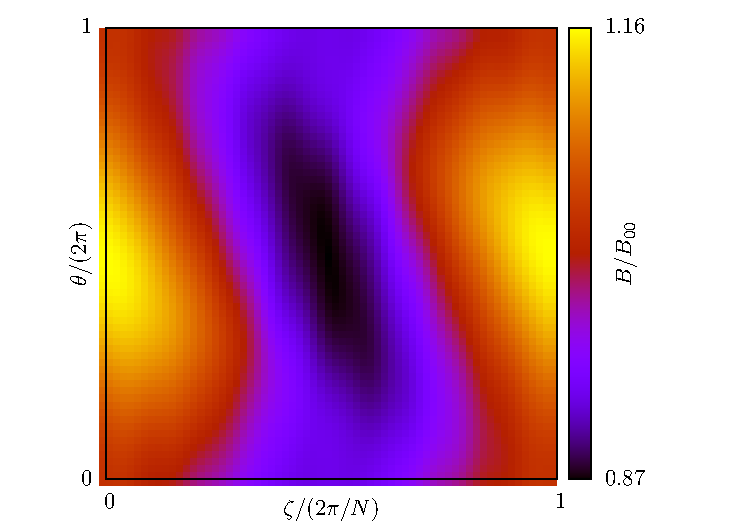
\includegraphics[angle=0,width=0.45\columnwidth]{figures/Bw7x.pdf}
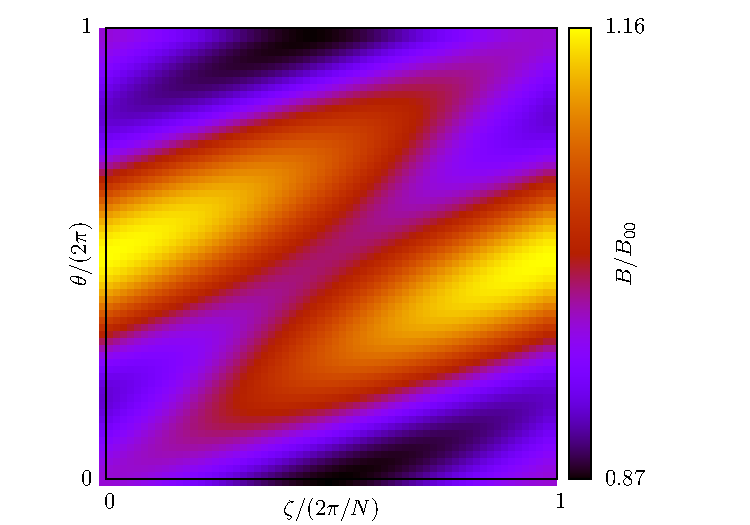
\includegraphics[angle=0,width=0.45\columnwidth]{figures/Blhd.pdf}
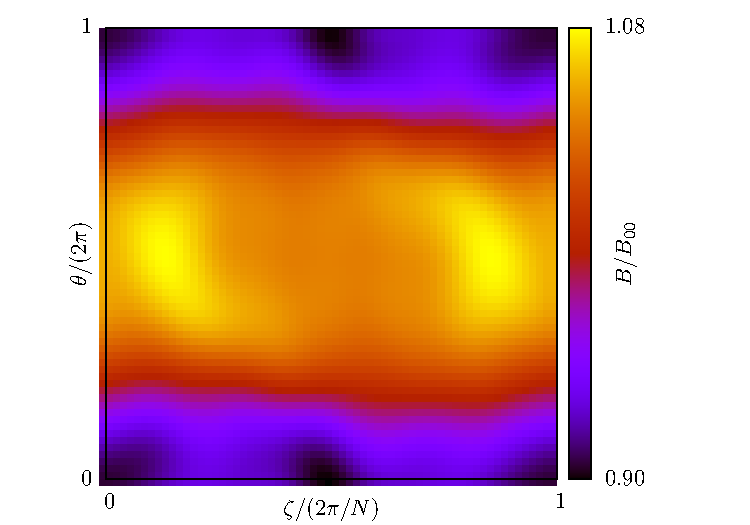
\includegraphics[angle=0,width=0.45\columnwidth]{figures/Bncsx.pdf}
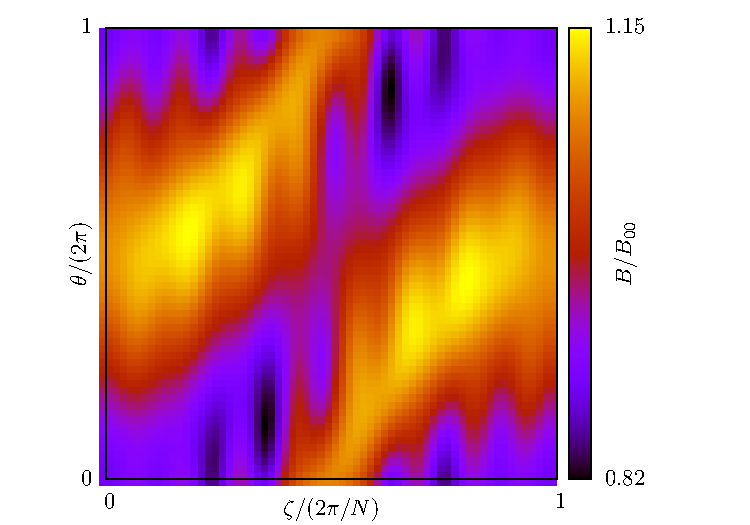
\includegraphics[angle=0,width=0.45\columnwidth]{figures/Btj2.pdf}
\caption{Magnetic field strength for surface $\psi/\psi_{LCFS}=0.5$ of the W7-X high-mirror configuration (top left), the LHD $R_{ax}=3.75\,$m configuration (top right), an NCSX equilibrium (bottom left) and the TJ-II standard configuration (bottom right).}
\label{FIG_MAP}
\end{figure}

\footnote{The input and output files of these simulations are provided in folder 'KNOSOS/TESTS/MONO', so that the user can reproduce them.} In this section, we will show that~\KNOSOS~can be used for creating a \DKES-like database of monoenergetic transport coefficients at low collisionalities. We will compare our calculations with~\DKES, both in results and computing time. Let us first discuss the rationale behind the monoenergetic approach, which is not specific to~\DKES, and the particular simplifications involved in~\DKES. More details can be found in the overview paper~\citep{beidler2011icnts}.

Predictive transport simulations solve the energy transport equation for every species:
\begin{equation}
\frac{3}{2}\frac{\partial n_bT_b}{\partial t}+ \frac{1}{r}\frac{\partial}{\partial r}(r Q_b)= \fsa{P_b}\,,
\end{equation}
where $P_b$ is the net energy input to species $b$ and the energy flux $Q_b$ contains a turbulent contribution, at least close to the edge, that is currently provided by simplified models~\citep{turkin2011predictive}. Calculating the time evolution of the energy, as in~\citep{sunnpedersen2015op11}, or finding the steady-sate solution as in~\citep{geiger2014w7x}, requires evaluating the neoclassical contribution to $Q_b$ a large number of times. The monoenergetic approach, together with some simplifications to the drift-kinetic equation, provides a way out of solving the drift-kinetic equation many times.

Strictly speaking, monoenergetic transport coefficients can always be calculated if the velocity $v$ is a parameter in the drift-kinetic equation that is being solved, as in the case of equation~(\ref{EQ_NDKE}): one can rewrite
\begin{equation}
Q_b = \int_0^\infty\mathrm{d} v D_{11,b}\frac{m_bv^2}{2} F_{M,b} \Upsilon_b\frac{\partial\psi}{\partial r}
\end{equation}
as a {\textit{convolution}} of monoenergetic transport coefficients
\begin{equation}
D_{11,b} = 2\left(\frac{\partial r}{\partial\psi}\right)^2\left\langle\int_{B^{-1}_{{\rm max}}}^{B^{-1}}\mathrm{d}\lambda\frac{v^3 B}{|v_\parallel |}\frac{g_b}{F_{M,b}\Upsilon_b}\mathbf{v}_{D,b}\cdot\nabla\psi\right\rangle \,,
\label{EQ_D11}
\end{equation}
where $g_b$ is the solution of equation~(\ref{EQ_NDKE}). Up to this point, the reduction in computation time associated to the monoenergetic approach stems from the fact that $v$ is a parameter in equation (\ref{EQ_NDKE}), which is then easier to solve than a drift-kinetic equation with energy diffusion in the collision operator.

Additionally, some fundamental simplifications are done by~\DKES: instead of $Q_b$, it calculates
\begin{equation}
\hat Q_b=\fsa{\mathbf{\hat Q_b}\cdot\nabla r} = \int_0^\infty\mathrm{d} v \hat D_{11,b}\frac{m_bv^2}{2} F_{M,b} \Upsilon_b\frac{\partial\psi}{\partial r}\,,\label{EQ_HATQ}
\end{equation}
with 
\begin{equation}
\hat D_{11,b} = 2\left(\frac{\partial r}{\partial\psi}\right)^2\left\langle\int_{B^{-1}_{{\rm max}}}^{B^{-1}}\mathrm{d}\lambda\frac{v^3 B}{|v_\parallel |}\frac{\hat g_b}{F_{M,b}\Upsilon_b}\mathbf{v}_{M,b}\cdot\nabla\psi\right\rangle \,.
\end{equation}
Here, $\hat g_b$ is the solution of a modified version of equation~(\ref{EQ_NDKE}), simplified as
\begin{equation}
\hat I_{v_E,\alpha}(\alpha,\lambda)\partial_\alpha \hat g_b +  I_{v_{M,\psi}}(\alpha,\lambda) {v_{d,b}} F_{M,b}\Upsilon_b
= \nu_{\lambda,b} \partial_\lambda\left[ I_\nu(\alpha,\lambda) \partial_\lambda \hat g_b\right]\,.
\label{EQ_DKES}
\end{equation}
With respect to equations (\ref{EQ_NDKE}) and (\ref{EQ_D11}), we have set 
\begin{eqnarray}
\mathbf{v}_E\cdot\nabla\psi&=&0\,,\nonumber\\
I_{v_{M,\alpha}}&=&0\,,\nonumber\\
I_{v_{E,\psi}}&=&0\,,\label{EQ_BINTDKES}
\end{eqnarray}
and replaced $I_{v_{E,\alpha}}$ with
\begin{eqnarray}
\hat I_{v_{E,\alpha}}&=&\Psi_t'\partial_\psi\varphi_0\int_{l_{b_1}}^{l_{b_2}}\frac{B^2}{\fsa{B^2}} \frac{\mathrm{d}l}{\sqrt{1-\lambda B}}\,.
\end{eqnarray}
In other words, the effect of the tangential electric field and the tangential magnetic drift is ignored, and an incompressible $\mathbf{E}\times\mathbf{B}$ tangential drift is used (this last simplification is specific of~\DKES~and is not used by other codes in~\citep{beidler2011icnts}). While it is well known~\citep{calvo2017sqrtnu} that these effects need to be kept in the drift-kinetic equation for an accurate computation of the radial fluxes, there is a range of situations in which $\hat Q_b\approx Q_b$ (this will be discussed in detail in \S\ref{SEC_TANGVM}) and this inaccuracy allows for a very large reduction of the computing time. The reason is that, for a given flux-surface, when normalized by the plateau value
\begin{eqnarray}
\hat D_{11}^*&\equiv& \frac{\hat D_{11,b}}{D_{11,b}^p}\,,\nonumber\\
D_{11,b}^p&=& \frac{\pi v_{d,b}^2 R_0}{4v\iota}\,,
\end{eqnarray}
the transport coefficients $\hat D_{11}^*$ only depend on two $v$-dependent dimensionless parameters, the collisionality 
\begin{equation}
\nu_{*}=\frac{R_0\nu_\lambda}{\iota v}\,,
\end{equation}
and the normalized radial electric field
\begin{equation}
v_{E*}=\frac{E_r}{v B_{0,0}}\,.
\end{equation}
Here, $R_0$ is the major radius, and the main Fourier mode of $B$ (see \S\ref{SEC_DELTA}) is $B_{0,0}\sim 1\,$T in all the simulations presented in this paper. Since there is no species dependence, in the rest of the section, we follow the common practice of dropping the species index when discussing monoenergetic calculations. A predictive transport simulation thus requires to precompute a so-called database of (\DKES-like) monoenergetic coefficients $\hat D_{11}^*( \nu_*,v_{E*}$). Once this is done, the calculation of $\hat Q_b$ for given $n_b$, $T_b$ and $E_r$ using equation~(\ref{EQ_HATQ}) requires a few bidimensional interpolations and an integral in $v$. The problem then lies in the computation of the database $\hat D_{11}^*( \nu_*,v_{E*})$ for every new magnetic configuration, which typically takes hours, due to the poor convergence of~\DKES~(and most neoclassical codes~\citep{beidler2011icnts}) at low collisionalities. We will show that the bounce-average technique greatly reduces the computing time by using in~\KNOSOS~equation (\ref{EQ_DKES}) and comparing the results with~\DKES. Calculations without the simplifications made by~\DKES~are left for \S\ref{SEC_TANGVM}.

In order to illustrate the performance of~\KNOSOS~in a variety of three-dimensional configurations, we choose four very different types of stellarators. Figure~\ref{FIG_MAP} shows the map of the magnetic field strength on the flux-surface  $\psi/\psi_{LCFS}=0.3$ of the high-mirror configuration of the helias W7-X (top left), the $R_{ax}=3.75\,$m configuration of the heliotron LHD (top right), an equilibrium of NCSX close to  quasiaxisymmetry (bottom left) and the standard configuration of the heliac TJ-II~(bottom right)\citep{ascasibar2019iaea}. 

\begin{figure}
\centering
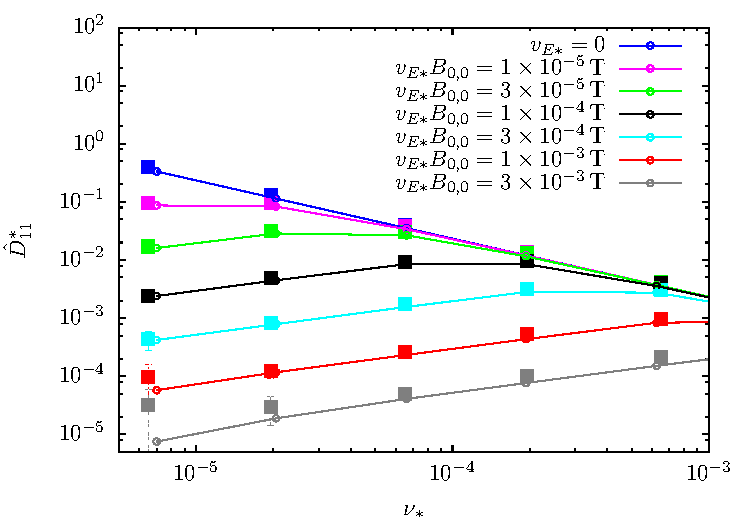
\includegraphics[angle=0,width=0.45\columnwidth]{figures/d11w7x.pdf}
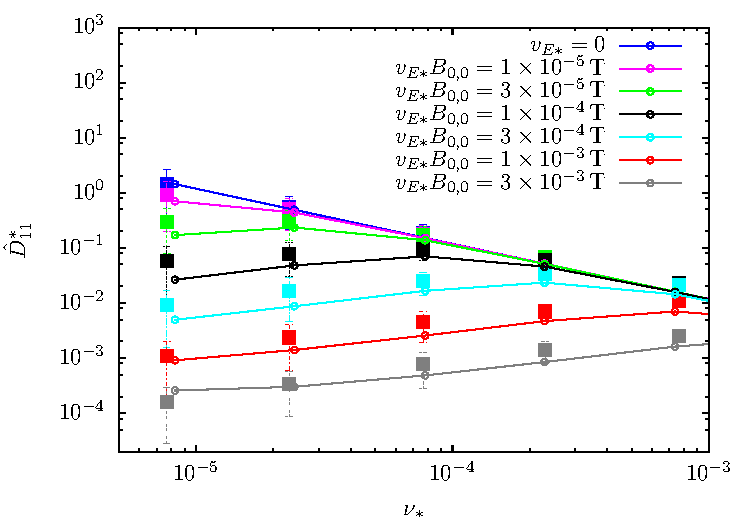
\includegraphics[angle=0,width=0.45\columnwidth]{figures/d11lhd.pdf}
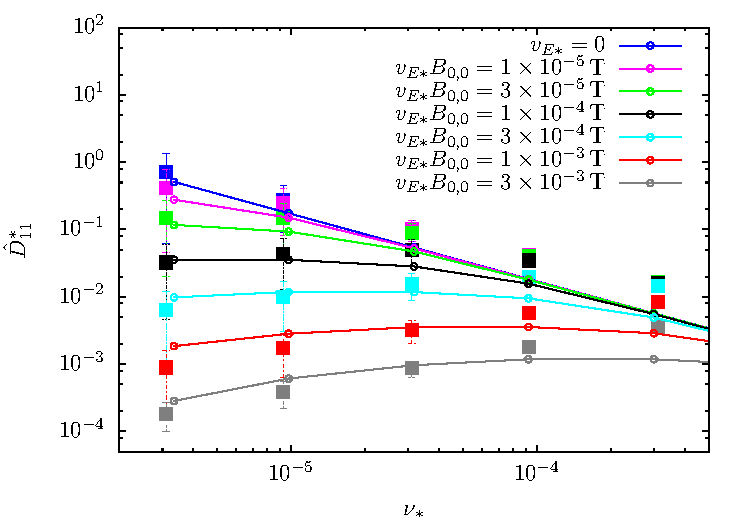
\includegraphics[angle=0,width=0.45\columnwidth]{figures/d11ncsx.pdf}
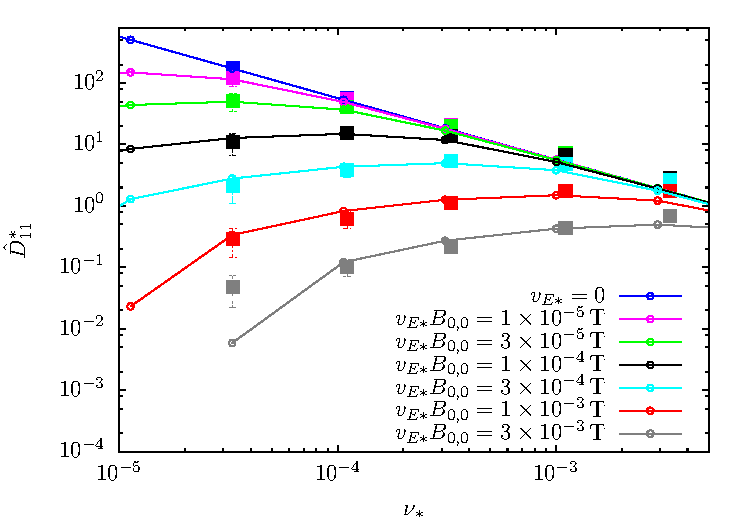
\includegraphics[angle=0,width=0.45\columnwidth]{figures/d11tj2.pdf}
\caption{Monoenergetic transport coefficients calculated with~\DKES~(full squares) and~\KNOSOS~(small open circles with lines) as a function of the collisionality at $\psi/\psi_{LCFS}=0.5$ surface of W7-X (top left), LHD (top right), NCSX (bottom left) and TJ-II (bottom right). The colour code is: $v_{E*}B_{0,0}=0$ (blue),  $1\times 10^{-5}\,$T (magenta),  $3\times 10^{-5}\,$T (green),  $1\times 10^{-4}\,$T (black),  $3\times 10^{-4}\,$T (cyan),  $1\times 10^{-3}\,$T (red),  and $3\times 10^{-3}\,$T (grey).}
\label{FIG_D11}
\end{figure}


Figure~\ref{FIG_D11} shows the first comparisons between~\KNOSOS~and~\DKES, in which the normalized monoenergetic transport coefficient $\hat D_{11}^*$ is calculated for several values of the collisionality and the normalized radial electric field.  Figure~\ref{FIG_D11} (top left) contains data for the W7-X high-mirror configuration, which we discuss in more detail. The expected $1/\nu$ dependence is observed at the highest collisionalities and, due only to the absence of tangential magnetic drift, for small values of $v_{E*}$. There is $\sqrt{\nu}$ characteristic behaviour elsewhere, with smaller levels of transport for larger $|E_r|$. The comparison between~\KNOSOS~and~\DKES~is satisfactory, with agreement within the error bars of the~\DKES~calculation, and only at the highest collisionalities, and for the largest values of $E_r$,  there are very small differences. The calculation for all the points of this case was made with ${\cal{N}}_\alpha=32$   and ${\cal{N}}_\lambda=64$, and it took $2.0$ seconds in a single standard CPU. Of this time, around $0.7$ seconds were used for setting the grid and performing the bounce-averages, and then it took less than $0.04$ seconds to calculate each point. This number may be reduced even further using smaller ${\cal{N}}_\lambda$ for the cases of largest collisionality and smallest radial electric field. In the $\sqrt{\nu}$ regime, transport is given by a small layer close to the boundary between passing and trapped particles. The size in $\lambda$ of this layer is proportional to $\sqrt{\nu_\lambda/E_r}$~\citep{calvo2017sqrtnu}, and this determines the required number of grid points ${\cal{N}}_\lambda$ in the low collisionality cases with radial electric field.
\begin{figure}
\centering
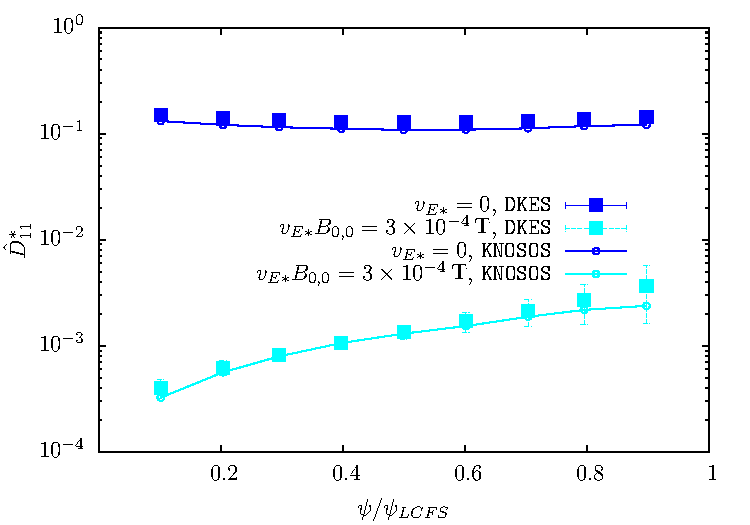
\includegraphics[angle=0,width=0.45\columnwidth]{figures/d11w7x_prof.pdf}
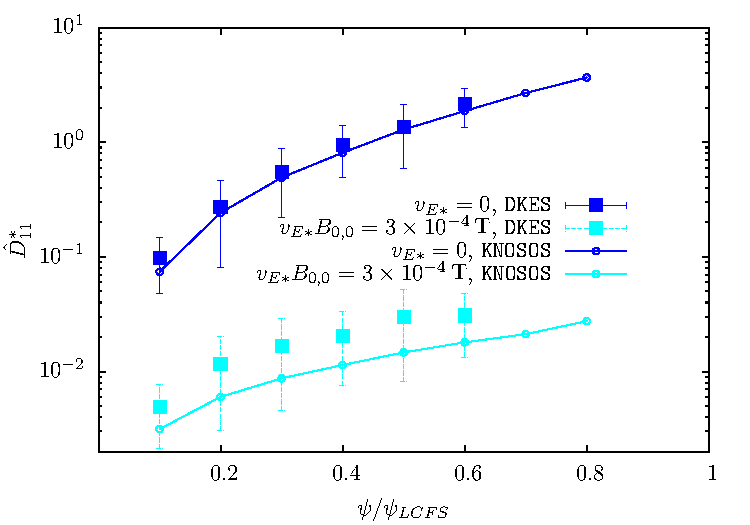
\includegraphics[angle=0,width=0.45\columnwidth]{figures/d11lhd_prof.pdf}
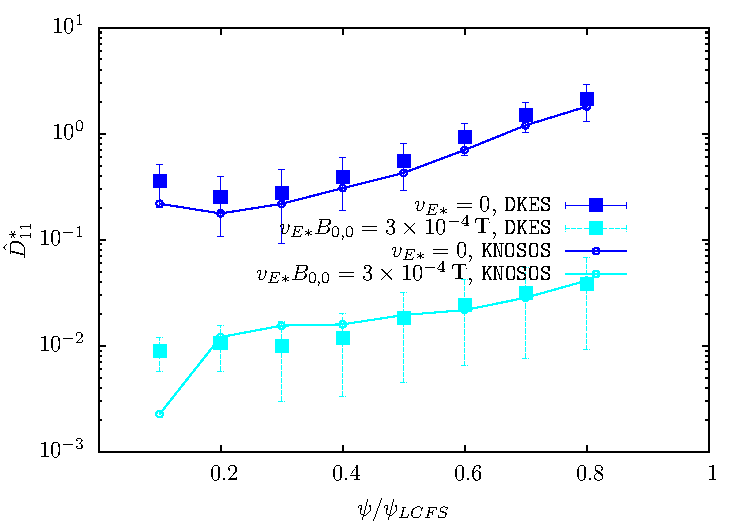
\includegraphics[angle=0,width=0.45\columnwidth]{figures/d11ncsx_prof.pdf}
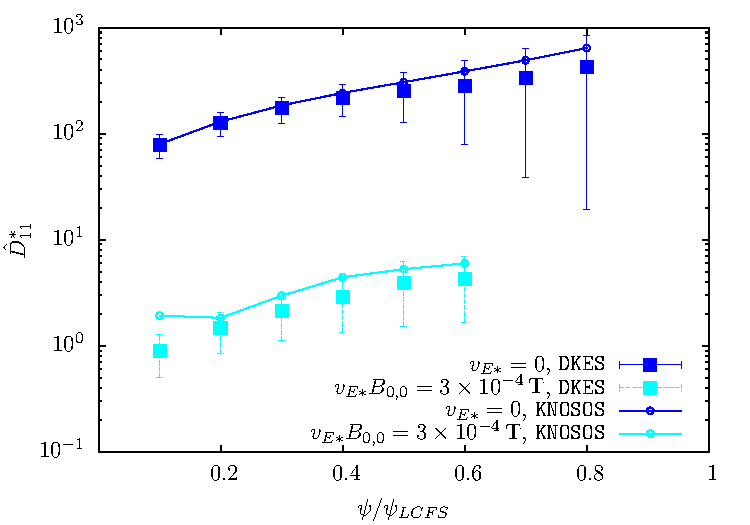
\includegraphics[angle=0,width=0.45\columnwidth]{figures/d11tj2_prof.pdf}
\caption{Radial profile of normalized monoenergetic transport coefficient calculated with~\DKES~(full squares) and~\KNOSOS~(small open circles with lines) for W7-X (top left), LHD (top right), NCSX (bottom left) and TJ-II (bottom right). Cyan corresponds to the $\sqrt{\nu}$ regime ($v_{E*}B_{0,0}=3\times 10^{-4}\,$T) and blue to the $1/\nu$ regime ($v_{E*}=0$).}
\label{FIG_D11PROF}
\end{figure}

Similar results can be seen for LHD in figure~\ref{FIG_D11} (top right). ${\cal{N}}_\alpha=32$  and ${\cal{N}}_\lambda=64$ grid points were used, and the total computation time was 2.1 seconds. For NCSX,  figure~\ref{FIG_D11} (bottom left), the agreement is good except for the higher collisionalities, where the $1/\nu$ regime should connect with a banana regime (see figure 15 of~\citep{beidler2011icnts}). This regime could be easily implemented in~\KNOSOS~following~\citep{landreman2012omni}. ${\cal{N}}_\alpha=32$  and ${\cal{N}}_\lambda=64$ grid points were used, and the total computation time was 1.0 seconds. Finally, figure~\ref{FIG_D11} (bottom right) contains the results for TJ-II, the hardest case due to its complicated magnetic geometry, see figure~\ref{FIG_MAP} (bottom right). ${\cal{N}}_\alpha=32$  and ${\cal{N}}_\lambda=128$ were used, and the simulation took 157 seconds.  Here, one can see more clearly that the cases deeper in the $\sqrt{\nu}$ regime are more difficult to converge, and indeed the points corresponding to $v_{E*}B_{0,0} \geq 10^{-3}\,$T and $\nu_*< 10^{-4}$ are barely converged. The rest of the simulations agree with~\DKES~and reach even lower collisionalities than those typically required for describing a TJ-II plasma, whose ion temperature never exceeds a few hundred eV.
 


Figure~\ref{FIG_D11PROF} contains, for each of the four configurations, radial profiles of the transport coefficient $\hat D^*_{11}$ for two cases, $v_{E*}=0$ and $v_{E*}B_{0,0}=3\times 10^{-4}\,$T, for a given collisionality.  They are meant to represent the level of transport in the $1/\nu$ regime ($\hat D^*_{11}$ is by definition proportional to $\epsilon_{eff}^{3/2}$, being $\epsilon_{eff}$ the effective ripple) and  the $\sqrt{\nu}$ regime, respectively. We choose $\nu_*=2\times 10^{-5}$  for W7-X (top left) and LHD (top right), $\nu_*=10^{-5}$ for NCSX (bottom left) and $\nu_*=3\times 10^{-5}$ for TJ-II (bottom right). It can be observed that the good agreement holds for all cases at all radial positions. The comparison of the different parts of figure~\ref{FIG_D11PROF} provides additional information that may be relevant when devising a stellarator optimization strategy: in general, configurations with lower $1/\nu$ transport show lower $\sqrt{\nu}$ transport as well. This is not surprising considering that both quantities are connected to the bounce-averaged radial component of the magnetic drift, which appears in the source of the drift-kinetic equation~(\ref{EQ_DKEFINAL}) in both regimes, and which is in turn proportional to the variation of the second adiabatic invariant on the flux-surface, $\partial_\alpha J$. Inasmuch as the optimization procedure actually reduces the size of $\partial_\alpha J$, both the $1/\nu$ and $\sqrt{\nu}$ (and superbanana-plateau) regimes will generally be optimized. Nevertheless, using directly the effective ripple as figure of merit of neoclassical transport does not automatically guarantee a reduction of $\partial_\alpha J$, and the $\sqrt{\nu}$ transport may remain unoptimized. Figure~\ref{FIG_D11PROF}  (top) may represent an example of this situation: while this W7-X configuration is designed to have low level of $1/\nu$ transport at an intermediate radial position (where the plasma volume is relatively large and neoclassical transport is expected to be at least comparable to anomalous transport), the $\sqrt{\nu}$ transport is smallest exactly at the magnetic axis. We will argue the relevance of optimizing transport regimes of collisionality lower than the $1/\nu$, which has now become possible with~\KNOSOS, in the next section.


%%%%%%%%%%%%%%%%%%%%%%%%%%%%%%%%%%%%%%%%%%%%%%%%%%%%%%%%%%%%%%%%%%%%%%%%%%%%%%%%%%%%%%%%%%%%%%%%%%%%%%%%%%%%%%%%%%%

\section{Effect of the tangential magnetic drift on the radial transport of energy}\label{SEC_TANGVM}

%%%%%%%%%%%%%%%%%%%%%%%%%%%%%%%%%%%%%%%%%%%%%%%%%%%%%%%%%%%%%%%%%%%%%%%%%%%%%%%%%%%%%%%%%%%%%%%%%%%%%%%%%%%%%%%%%%%

\footnote{The input and output files of these simulations are provided in folder 'KNOSOS/TESTS/AMB', so that the user can reproduce them.} In \S\ref{SEC_DKES}, we have shown solutions of equation~(\ref{EQ_DKES}), a simplified drift-kinetic equation that is not accurate when the tangential components of the magnetic drift and of the electric field play a role. In this section, we will demonstrate the importance of solving equation~(\ref{EQ_NDKE}) instead of equation~(\ref{EQ_DKES}), i.e., of computing $Q_b$ and not $\hat Q_b$, when calculating the radial energy flux in real plasmas. It must be noted that the solution of equation~(\ref{EQ_NDKE}) with~\KNOSOS~is not computationally more expensive than that of equation (\ref{EQ_DKES}): in the superbanana-plateau regime, that may arise in the presence of the tangential magnetic drift for certain values of $E_r$, transport is dominated by a resonant layer whose size decreases with $(\nu_\lambda/E_r)^{1/3}$, i.e., slower than the boundary layer that determines the $\sqrt{\nu}$ transport~\citep{calvo2017sqrtnu}. Calculating $Q_b$ instead of $\hat Q_b$ does not require a larger value of ${\cal{N}}_\lambda$ in general.

In this section, we focus on characterizing the effect of the tangential magnetic drift for the particular case of $\varphi_1=0$. We advance one of the salient results: this effect will be non-negligible even at not very low collisionalities. The reason is that the calculation of the energy flux for a given plasma, characterized by the kinetic profiles, requires the solution of the drift-kinetic equation for several values of the velocity, see equation~(\ref{EQ_CONV}), with the normalized particle energy $(v/v_{th,b})^2$ spanning several orders of magnitude. This means that, even if the thermal particles are in $1/\nu$ regime, there are particles with higher $v$ that are in lower collisionality regimes. 

Figure~\ref{FIG_QER1} contains simulations for the high-mirror configuration of W7-X at $\psi/\psi_{LCFS}=0.25$, which corresponds to $r/a=0.5$. We choose a pure hydrogen plasma, with $n_e=8.0\times 10^{19}\,$m$^{-3}$, $\partial_r n_e/n_e=-2.0\,$m$^{-1}$, $T_e = T_i = 4.0\,$keV, $\partial_r T_e/T_e =\partial_r T_i/T_i = -3.0\,$m$^{-1}$. These are values comparable to those measured in high-performance OP1.2 plasmas of W7-X~\citep{klinger2019op12} in the region of crossover between positive and negative radial electric field, corresponding to electron and ion root solutions of the ambipolarity equation~\citep{pablant2019ionroot}. In these plasmas, neoclassical transport calculated neglecting the tangential magnetic drift typically accounts for around half the total experimental transport. Figure~\ref{FIG_QER1} (top) contains a plot, in logarithmic scale, of the ion and electron radial energy flux as a function of the radial electric field. Empty and full blue boxes correspond to $\hat Q_i$ and $Q_i$ respectively, both calculated with~\KNOSOS. We immediately see that $\hat Q_i$ overestimates the radial energy flux at small values of the radial electric field, specially at $E_r = 0$ (strictly the only point of the figure where $\hat Q_i$ is proportional to $\varepsilon_{eff}^{3/2}$). The tangential drifts make the ion flux decrease, differently in the case of $\hat Q_i$ and $Q_i$, as we will discuss below. Finally, empty and full red boxes correspond to $\hat Q_e$ and $Q_e$ calculated with~\KNOSOS. In this plot, is difficult to notice any difference between the different electron calculations. Figure~\ref{FIG_QER1} (top) contains additional black lines that are the result of combining calculations with~\DKES~and~\KNOSOS. We will leave the discussion of these results for the end of the section.

Figure~\ref{FIG_QER1} (bottom) contains a blowup in linear scale of the most relevant range of the data in figure~\ref{FIG_QER1} (top). Here, the effect of the tangential magnetic drift on the energy flux can be observed more clearly: the size of the peak at small $|E_r|$ is reduced and displaced to positive (negative) values in the case of electrons (ions). The effect is larger for the ions due to their larger normalized Larmor radius $\rho_{i*}$, which makes them leave the $1/\nu$ regimes at relatively higher collisionalities. We have mentioned that these plasmas are close to the crossover between ion and electron root, and this figure can help us discuss some features of transport in both situations. In electron root, the radial electric field is expected to be positive and large, and the electrons are expected to give the largest contribution to energy transport. According to figure~\ref{FIG_QER1} (bottom), $Q_e$ provides a minor, although systematic, correction to $\hat Q_e$, below 10\% for this plasma profiles and configuration. The situation is different in ion root, typically characterized by a negative radial electric field that is small in size, and dominant ion transport. Here, including the tangential magnetic drift can lead to large corrections, above 50\% in some cases.

For the sake of completeness, figure~\ref{FIG_QER2} contains two more cases. In figure~\ref{FIG_QER2} (top) we repeat the calculation for a W7-X plasma of much higher collisionality, choosing $n_e=1.6\times 10^{20}\,$m$^{-3}$, $\partial_r n_e/n_e=-2.0\,$m$^{-1}$, $T_e = T_i = 2.5\,$keV, $\partial_r T_e/T_e =\partial_r T_i/T_i = -3.0\,$m$^{-1}$. We first note that the electrons are deep in the $1/\nu$ regime, since $\nu_{e*}=3.4\times 10^{-2}$ and $\rho_{e*}=1.4\times 10^{-5}$. Nevertheless, $Q_e(E_r)$ does not show the linear dependence expected when the $1/\nu$ dominates. This is an indication of what we advanced at the beginning of this section: even in plasmas nominally in the $1/\nu$ regime, the contribution of the $\sqrt{\nu}$ regime is not negligible, and should not be neglected in the optimization procedure. For the ions, even at these higher collisionalities and low temperatures, $\nu_{i*} = 1.6\times 10^{-2}$ is not much larger than $\rho_{i*} = 6.0\times 10^{-4}$ divided by the inverse aspect ratio. This means that, for ions slightly more energetic than the thermal ions, the tangential magnetic drift is relevant at small values of $|E_r|$~\citep{calvo2018jpp}. Figure~\ref{FIG_QER2} (top) shows indeed systematic differences between $\hat Q_i$ and $Q_i$. 

Finally, figure~\ref{FIG_QER2} (bottom) contains a calculation with the same kinetic profiles of figure~\ref{FIG_QER1} (top) for the inward-shifted configuration of LHD. It can be observed that the effects discussed in figure~\ref{FIG_QER2} (top) are even more pronounced, to the extent of changing qualitatively the $Q_b(E_r)$ dependence (and making it more similar to that reported in~\citep{matsuoka2015tangential}: while practically any increase of $|E_r|$ causes a reduction of $Q_i$ in W7-X, this is not the case for LHD. For finite ion-root values of $E_r$, $Q_i(E_r)$ has a peak whose height is determined by superbanana-plateau transport. 

In light of these results, two comments related to stellarator optimization can be made. First, the fact that the monoenergetic transport coefficients respond to small tangential $\mathbf{E}\times\mathbf{B}$ drifts differently in the inward-shifted LHD, with respect to other configurations, was already discussed in~\citep{beidler2011icnts}, and it can be observed more clearly when calculating the energy flux including the tangential magnetic drift. We also note that part of the neoclassical optimization of W7-X comes from its large aspect-ratio, which tends to make the tangential magnetic drift smaller, when compared with the $E\times B$ drift. It is then clear than a systematic study of the different low-collisionality regimes, and their different configuration dependence, should be addressed when devising an stellarator optimization strategy. Second, a comprehensive optimization strategy will involve, at least, solving energy transport consistently with ambipolarity and quasineutrality. Along this section, we have compared $Q$ and $\hat Q$ at fixed $E_r$, but a more systematic study applied to real discharges of W7-X, including the experimental validation of $E_r$ predictions, is ongoing~\citep{carralero2019irw}.

Let us finally discuss the black lines of figures~\ref{FIG_QER1} and~\ref{FIG_QER2}, which correspond to combining simulations of~\DKES~and~\KNOSOS. As we have argued at the beginning of this section, calculating the radial energy flux requires solving the drift-kinetic equation for velocities $(v/v_{th,b})^2$ spanning from $\sim 10^{-2}$ to $\sim 10^{2}$, typically. Similarly to what we discussed for $v\gg v_{th,b}$, this means that particles with $v\ll v_{th,b}$ could be in the plateau regime, and they would not be described by equation~(\ref{EQ_NDKE}). In order to quantify this effect, and to show that it is negligible for the high-performance plasmas of W7-X, we perform calculations of $Q_i(E_r)$ and $Q_e(E_r)$ combining~\KNOSOS~with~\DKES. This can be done by rewriting equation~(\ref{EQ_GAMMAQ}) as
\begin{equation}
Q_b = D_{11,b}^p\int_0^\infty\mathrm{d} v \left[ H(v_0-v) \hat D^*_{11}(v) + H(v-v_0) D^*_{11}(v) \right] \frac{m_bv^2}{2}  F_{M,b} \Upsilon_b\,,
\label{EQ_DKESpKNOSOS}
\end{equation}
where $H$ is the Heaviside function, $v_0$ is a cut-off velocity, $\hat D^*_{11}(v)$ comes from~\DKES~in this case and
\begin{equation}
D^*_{11}(v) = \frac{D_{11,b}}{D_{11,b}^p}
\end{equation}
from~\KNOSOS. The latter is calculated according to equation~(\ref{EQ_D11}) solving the drift-kinetic equation that is correct at low collisionalities with $\varphi_1$ set to zero. In other words, monoenergetic transport coefficients $\hat D^*_{11}$ coming from~\DKES~are used above certain collisionality when performing the velocity integral and monoenergetic transport coefficients $D^*_{11}$ coming from~\KNOSOS~are used below that collisionality. The cut-off velocity $v_0$ must correspond to particles in the $1/\nu$ regime, which is correctly described by the two codes. This guarantees that both codes are employed in the parameter region where they are accurate (and fast).

In figures~\ref{FIG_QER1} and \ref{FIG_QER2} (bottom), the black lines corresponding to using equation~(\ref{EQ_DKESpKNOSOS}) barely separate from the solution of equation~(\ref{EQ_NDKE}). This means that the contribution of the plateau regime to the energy flux is negligible. Only for ions in the presence of very negative values of the radial electric field, in the high-density W7-X calculation, starts the black line to separate from the blue signs. This is to be expected: due to the approximate (exact in the case of $\hat Q_i$) $|E_r|^{-3/2}$-dependence of the transport coefficients in the $\sqrt{\nu}$, the contribution of low collisionalities to transport is reduced for very large values of $|E_r|$, and therefore the contribution of the plateau becomes non-negligible.

\begin{figure}
\centering
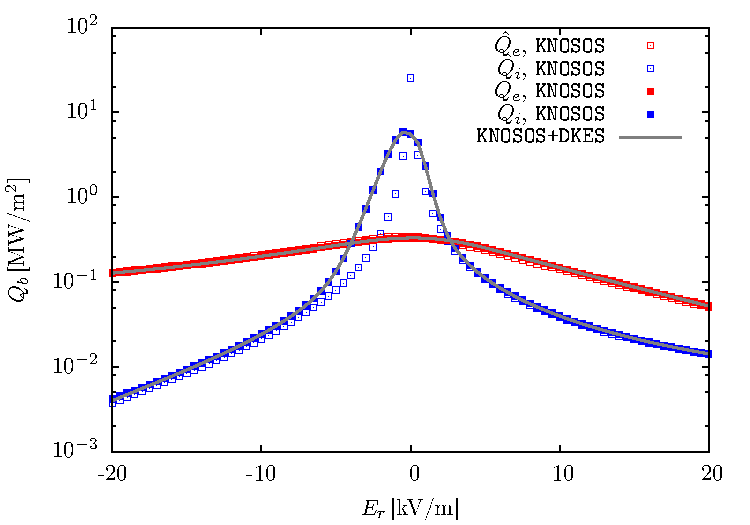
\includegraphics[angle=0,width=0.6\columnwidth]{figures/QEr.pdf}
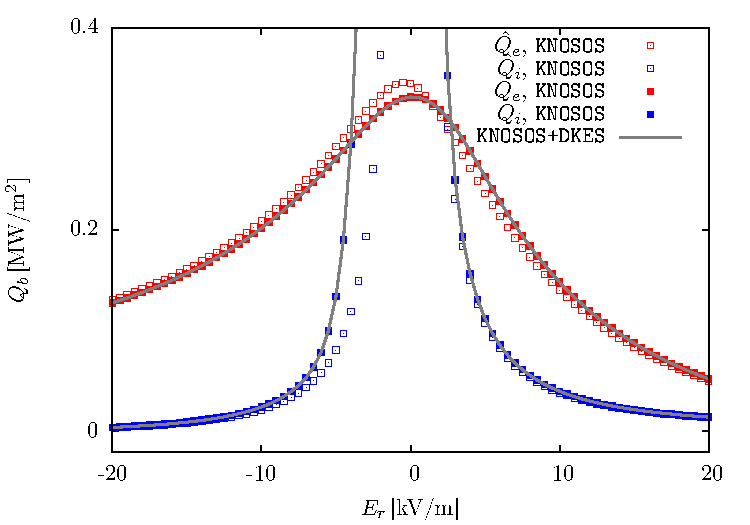
\includegraphics[angle=0,width=0.6\columnwidth]{figures/QEr_nolog.pdf}
\caption{Radial energy flux as a function of the radial electric field for a W7-X high-performance plasma: logarithmic (top) and linear (bottom) scale.}
\label{FIG_QER1}
\end{figure}

\begin{figure}
\centering
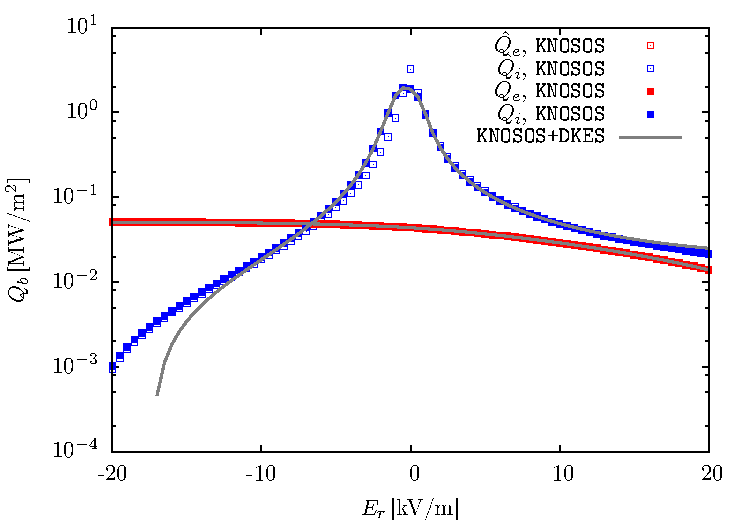
\includegraphics[angle=0,width=0.6\columnwidth]{figures/QEr_highn.pdf}
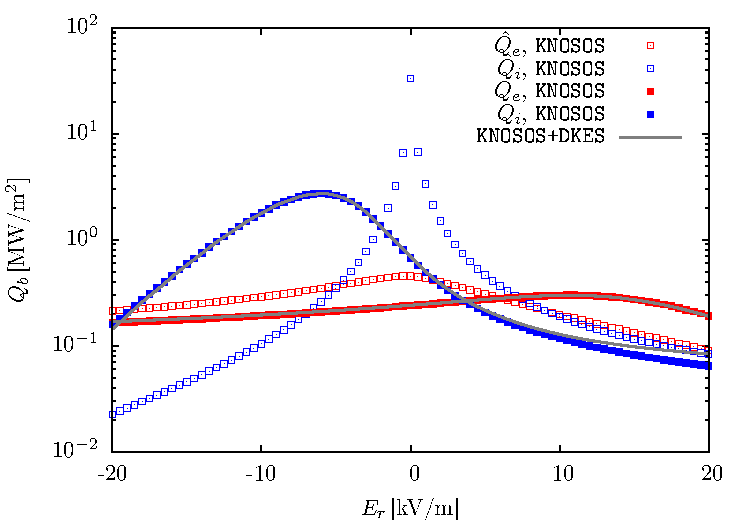
\includegraphics[angle=0,width=0.6\columnwidth]{figures/QEr_lhd.pdf}
\caption{Radial energy flux as a function of the radial electric field for a W7-X high density plasma (top) and an LHD plasma (bottom).}
\label{FIG_QER2}
\end{figure}

%%%%%%%%%%%%%%%%%%%%%%%%%%%%%%%%%%%%%%%%%%%%%%%%%%%%%%%%%%%%%%%%%%%%%%%%%%%%%%%%%%%%%%%%%%%%%%%%%%%%%%%%%%%%%%%%%%%

\section{Tangential electric field}\label{SEC_EUTERPE}

%%%%%%%%%%%%%%%%%%%%%%%%%%%%%%%%%%%%%%%%%%%%%%%%%%%%%%%%%%%%%%%%%%%%%%%%%%%%%%%%%%%%%%%%%%%%%%%%%%%%%%%%%%%%%%%%%%%

\begin{figure}
\begin{center}
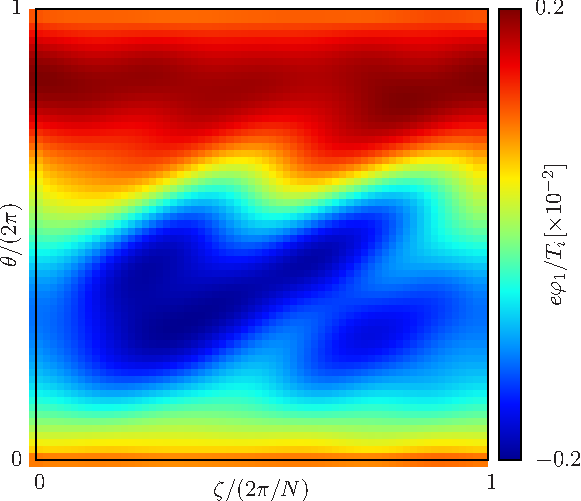
\includegraphics[width=0.3\columnwidth,angle=0]{figures/euterpeAIII02}
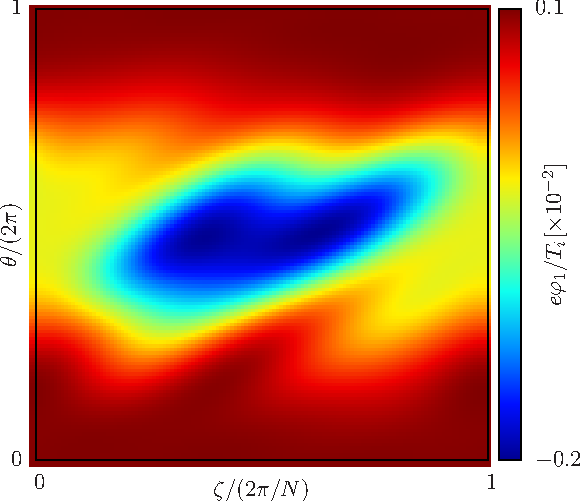
\includegraphics[width=0.3\columnwidth,angle=0]{figures/knososeutAIII02}
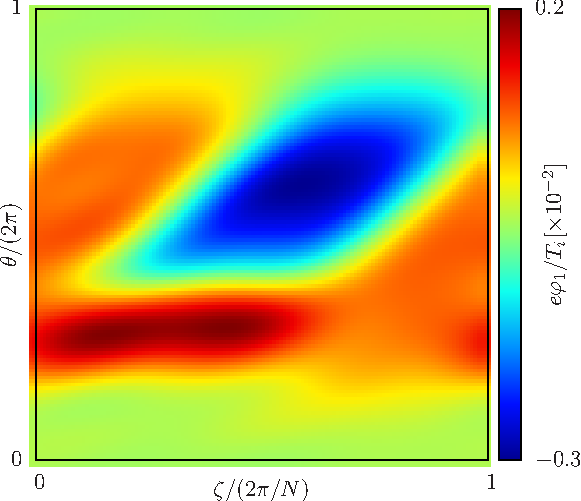
\includegraphics[width=0.3\columnwidth,angle=0]{figures/knososAIII02}

\

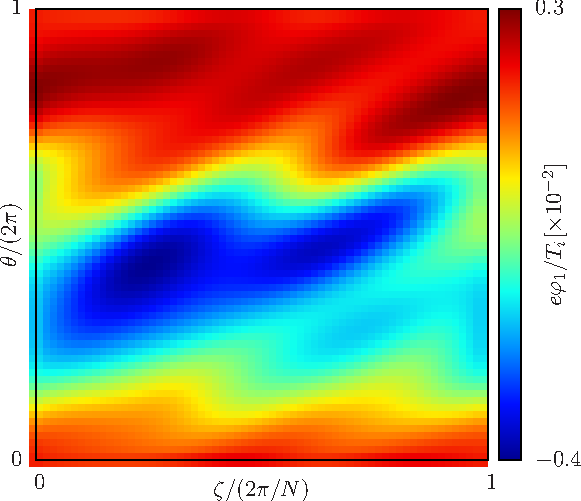
\includegraphics[width=0.3\columnwidth,angle=0]{figures/euterpeAIII04}
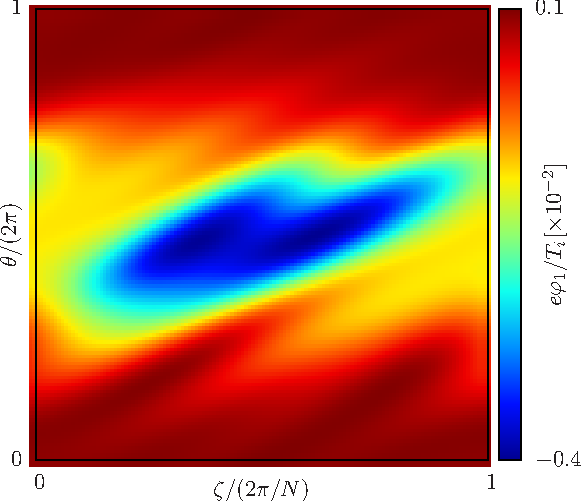
\includegraphics[width=0.3\columnwidth,angle=0]{figures/knososeutAIII04}
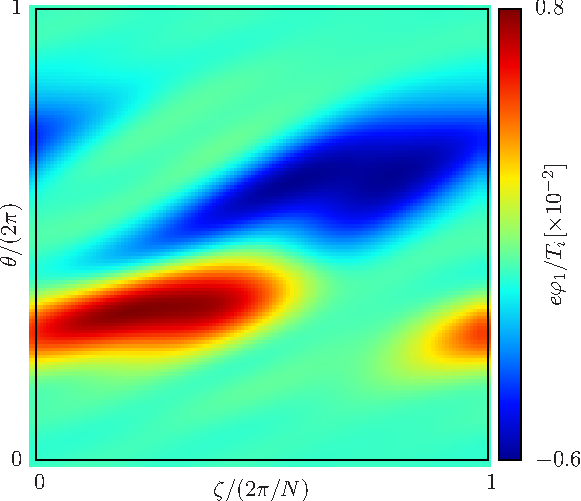
\includegraphics[width=0.3\columnwidth,angle=0]{figures/knososAIII04}

\

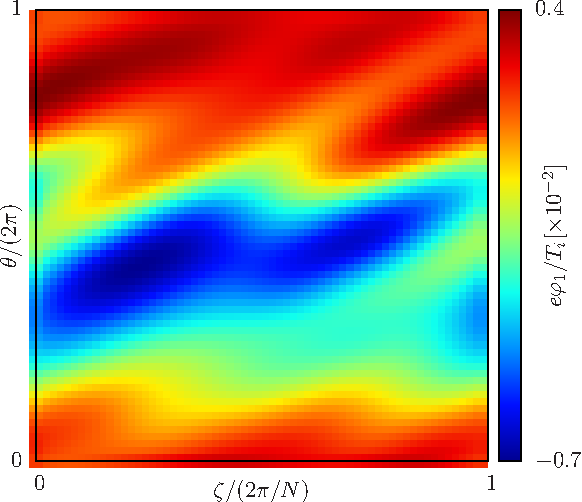
\includegraphics[width=0.3\columnwidth,angle=0]{figures/euterpeAIII06}
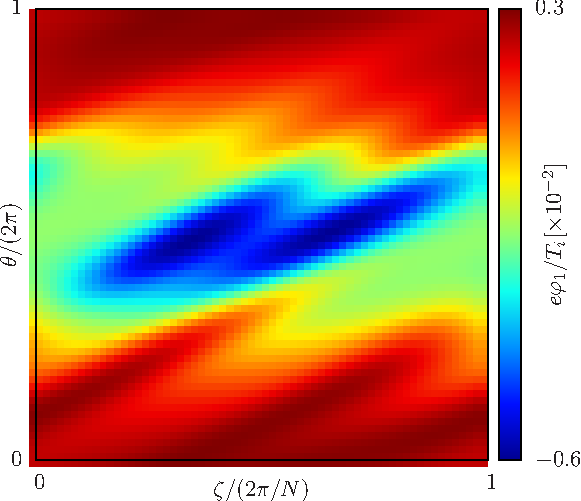
\includegraphics[width=0.3\columnwidth,angle=0]{figures/knososeutAIII06}
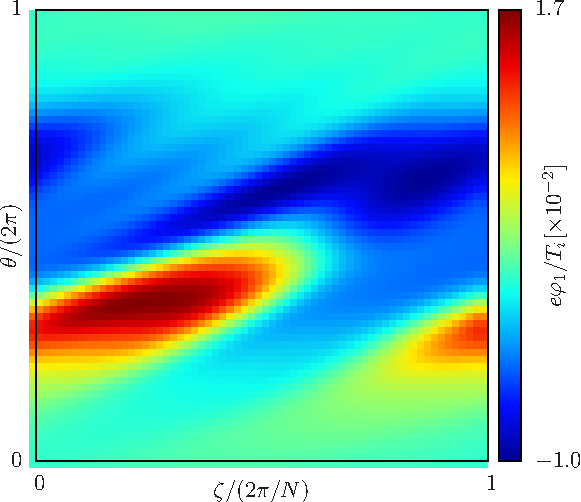
\includegraphics[width=0.3\columnwidth,angle=0]{figures/knososAIII06}

\

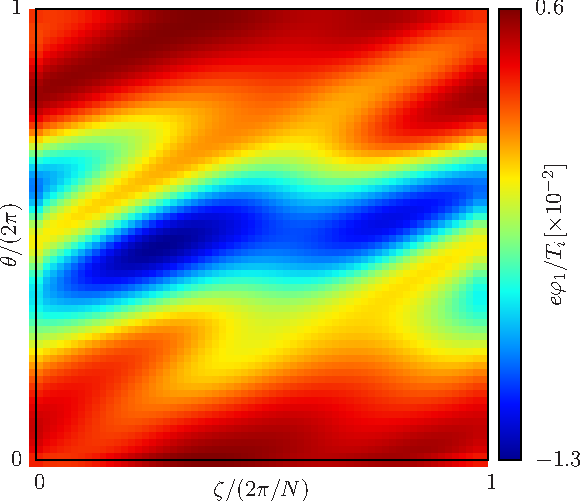
\includegraphics[width=0.3\columnwidth,angle=0]{figures/euterpeAIII08}
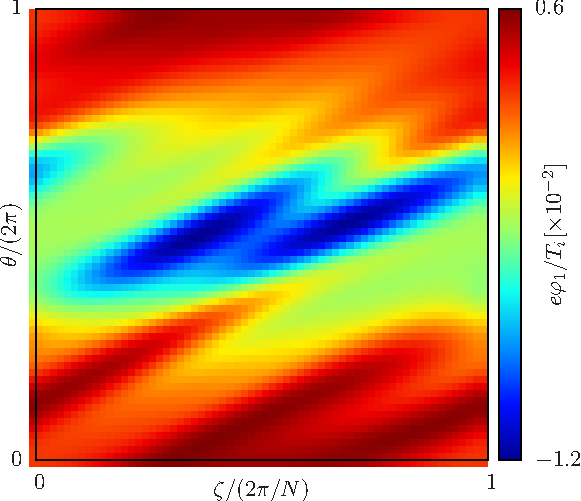
\includegraphics[width=0.3\columnwidth,angle=0]{figures/knososeutAIII08}
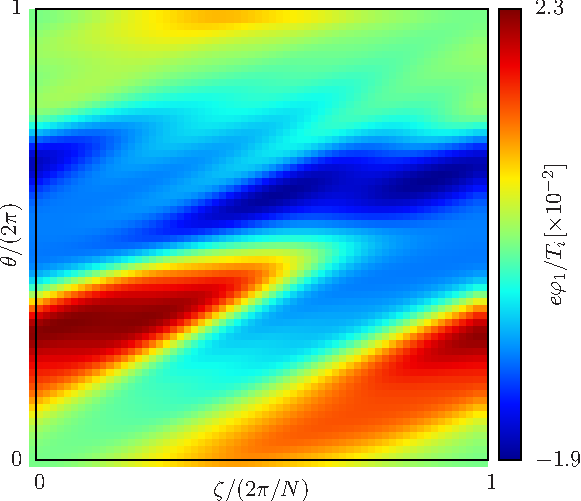
\includegraphics[width=0.3\columnwidth,angle=0]{figures/knososAIII08}
\end{center}
\caption{Electrostatic potential variation on the flux-surface calculated fort the LHD plasma with \texttt{EUTERPE} (left) and \texttt{KNOSOS} neglecting (center) and including (right) the tangential magnetic drift. The four rows correspond to radial positions $r/a\,=\,$0.2, 0.4, 0.6 and 0.8.}
\label{FIG_PHI1LHD}
\end{figure}

\begin{figure}
\begin{center}
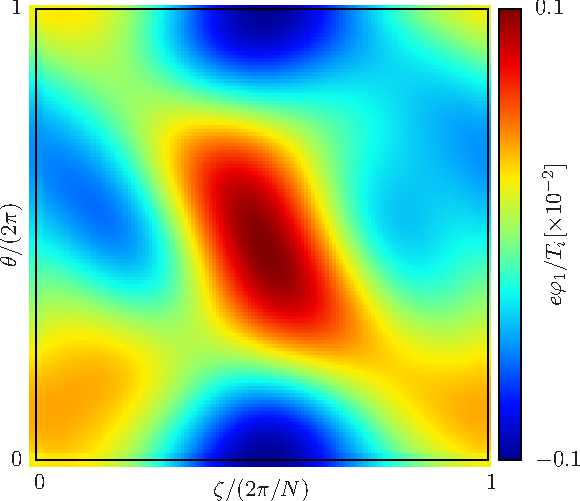
\includegraphics[width=0.3\columnwidth,angle=0]{figures/euterpeIV02}
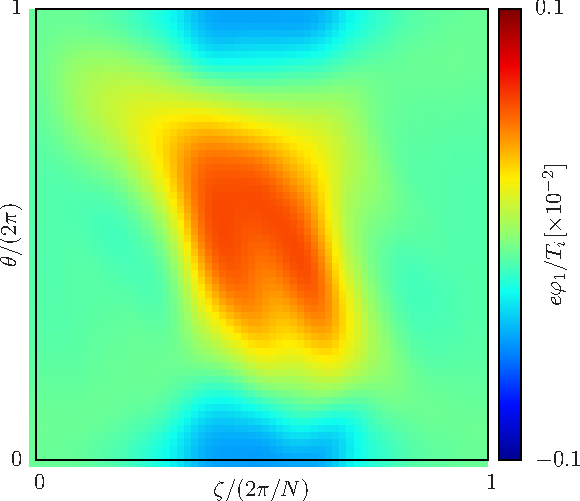
\includegraphics[width=0.3\columnwidth,angle=0]{figures/knososeutIV02}
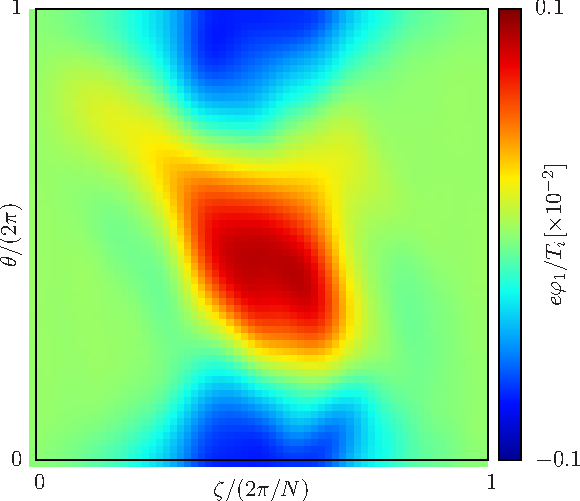
\includegraphics[width=0.3\columnwidth,angle=0]{figures/knososIV02}

\

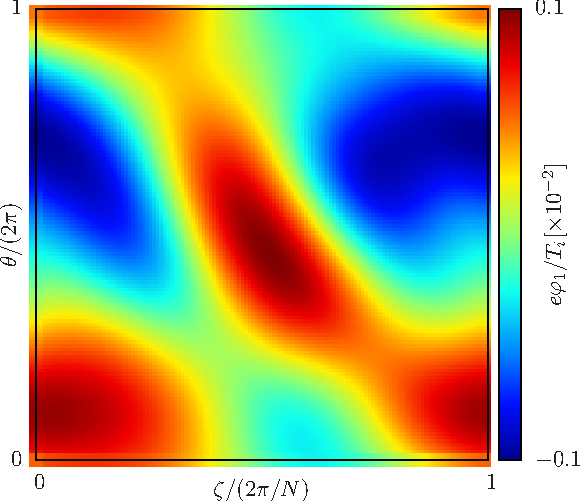
\includegraphics[width=0.3\columnwidth,angle=0]{figures/euterpeIV04}
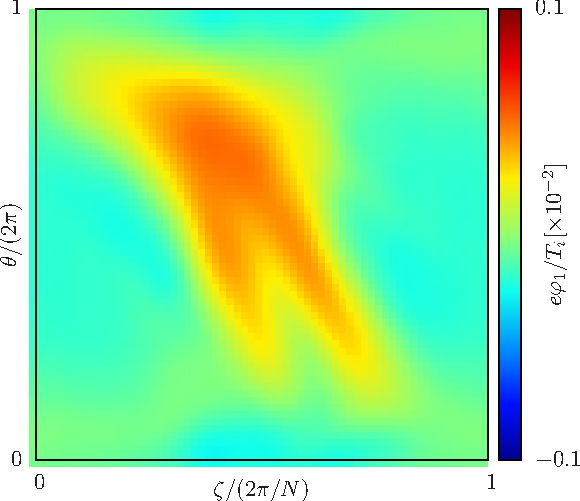
\includegraphics[width=0.3\columnwidth,angle=0]{figures/knososeutIV04}
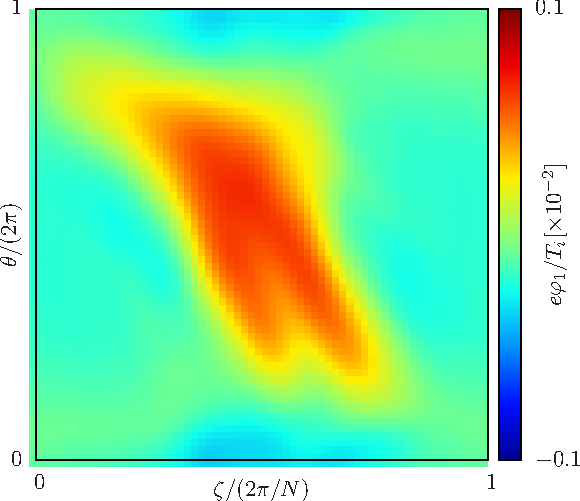
\includegraphics[width=0.3\columnwidth,angle=0]{figures/knososIV04}

\

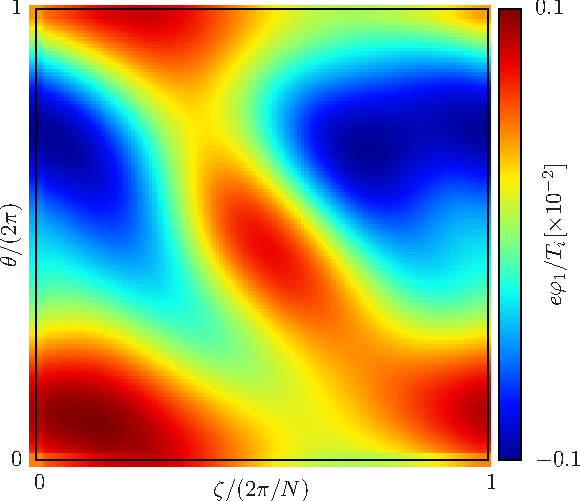
\includegraphics[width=0.3\columnwidth,angle=0]{figures/euterpeIV06}
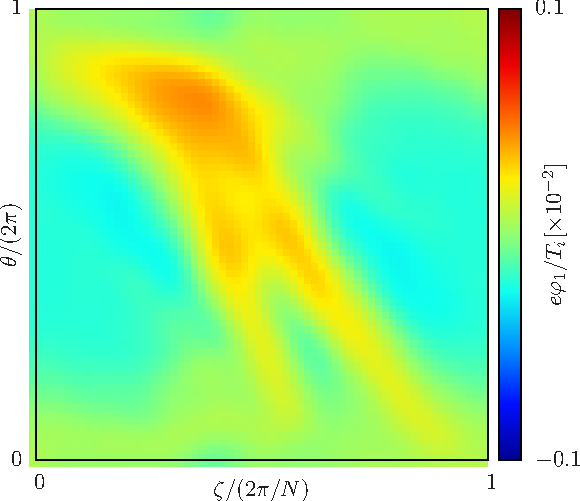
\includegraphics[width=0.3\columnwidth,angle=0]{figures/knososeutIV06}
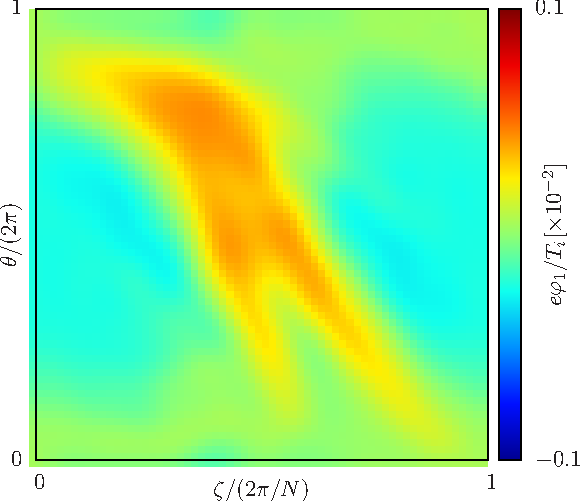
\includegraphics[width=0.3\columnwidth,angle=0]{figures/knososIV06}

\

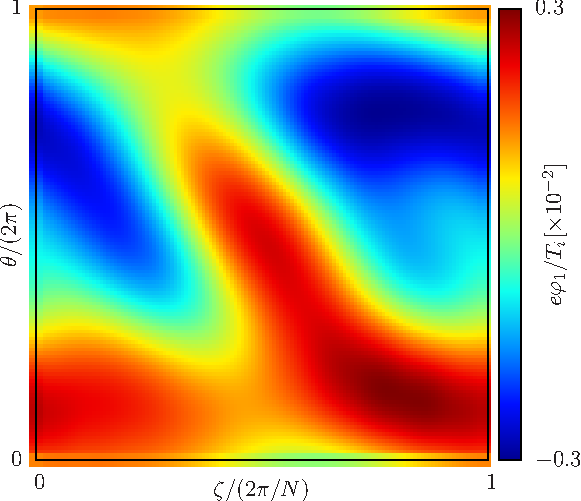
\includegraphics[width=0.3\columnwidth,angle=0]{figures/euterpeIV08}
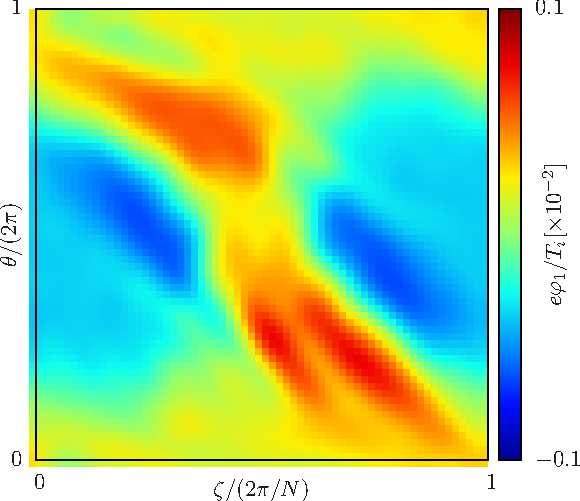
\includegraphics[width=0.3\columnwidth,angle=0]{figures/knososeutIV08}
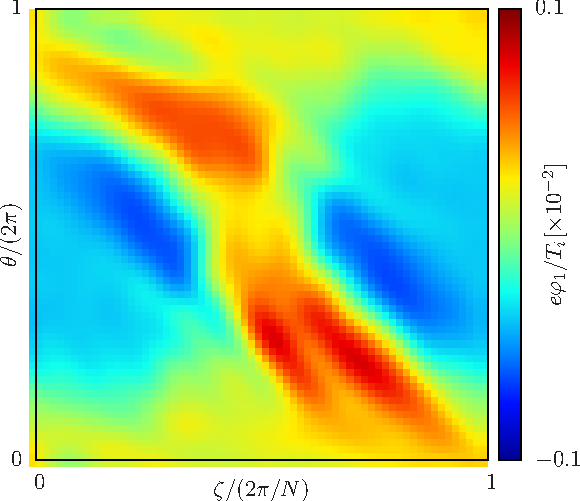
\includegraphics[width=0.3\columnwidth,angle=0]{figures/knososIV08}
\end{center}
\caption{Electrostatic potential variation on the flux-surface calculated fort the W7X plasma with \texttt{EUTERPE} (left) and \texttt{KNOSOS} neglecting (center) and including (right) the tangential magnetic drift. The four rows correspond to radial positions $r/a\,=\,$0.2, 0.4, 0.6 and 0.8.}
\label{FIG_PHI1W7X}
\end{figure}

\footnote{The input and output files of these simulations are provided in folder 'KNOSOS/TESTS/QN', so that the user can reproduce them.} Neoclassical physics gives rise to $\varphi_1$, and the associated tangential electric field produces radial drifts in all species. This is the reason why we need to solve consistently the drift-kinetic equations of the bulk species and quasineutrality~\citep{calvo2017sqrtnu}, but the effect is more relevant for impurities, due to their larger charge number, changing even qualitatively transport~(e.g. making it depend on the radial electric field in the so-called mixed collisionality regime~\citep{calvo2018nf,buller2018jpp}).  With impurity transport in mind, simulations of $\varphi_1$ for the stellarators W7-X, LHD and TJ-II have been performed in the last years with three codes,~\EUTERPE,~{\ttfamily SFINCS} and recently {\ttfamily FORTEC-3D}~\citep{regana2013euterpe,regana2017phi1,regana2018phi1,mollen2018phi1,fujita2019phi1}. Nevertheless, the number of simulations remains small because they are computationally very demanding, specially at low collisionalities. A more comprehensive study, including dependence on the configuration, collisionality, and bulk plasma profiles thus remains to be done.  In this section, we will show that~\KNOSOS~can reproduce the results of~\EUTERPE~(with adiabatic electrons and no tangential magnetic drift) and, by accounting for the effect of the tangential magnetic drift, describe stellarator regimes only simulated before for simplified geometries~\citep{calvo2018jpp,velasco2018phi1}. Since it can do so while keeping the computing time low, this opens the door to a number of new impurity transport studies. 

We start by reproducing the results of~\citep{regana2017phi1}, specifically of two low-collisionality plasmas of LHD and W7-X.  These are expected to be the plasma conditions of largest $e\varphi_1/T_i$ so that, even in optimized magnetic configurations, the effect on the radial transport of impurities may be large. It will be confirmed (as advanced in a previous work~\citep{velasco2018phi1} in a simplified calculation) that the inclusion of the tangential magnetic field leads to qualitative changes in $\varphi_1$, making it larger. Figure~\ref{FIG_PHI1LHD} shows the variation of the electrostatic potential on several flux-surfaces of the inward-shifted configuration of LHD for a low-collisionality plasma (described in~\citep{regana2017phi1}, termed AIII, and characterized by a small negative $E_r$). Each row corresponds to a different flux-surface, and each column to a different calculation method. Let us start by comparing the left column, calculated with~\EUTERPE, with the center column, calculated with~\KNOSOS~using equation (\ref{EQ_DKES}). The two methods should give the same results, and it can be observed that, although there are some differences, reasonable agreement between the two codes is obtained. It should be emphasized that differences in calculated values of $\varphi_1$ similar but smaller to those reported here, have been shown to produce negligible differences in impurity transport~\citep{velasco2018phi1}. If we now focus on the right column, we observe, as discussed in detail in~\citep{velasco2018phi1}, that the inclusion of the tangential produces relevant differences (in particular, more important than those between the left and center columns): the amplitude becomes larger, and the phase changes, with the angular dependence of $\varphi_1$ turning from being stellarator-symmetric (as expected for ions in the $\sqrt{\nu}$ regime), to not having definite symmetry (as corresponds to the superbanana-plateau regime~\citep{calvo2018jpp}).

Figure~\ref{FIG_PHI1W7X} contains a similar calculation performed for a low-collisionality plasma of W7-X (described in~\citep{regana2017phi1}, termed IV, and characterized by a larger negative $E_r$). Again, each row corresponds to a different flux-surface, and each column to a different calculation method. The comparison between~\EUTERPE~and~\KNOSOS~solving the same equation (left and center) is good close to the core, but it becomes slightly worse closer to the edge, where~\KNOSOS~underestimates the amplitude of $\varphi_1$. When the tangential magnetic drift is included (right), the results change very slightly in the core and do not change elsewhere. This feature is likely caused by the large radial electric field, which leaves the ions in the $\sqrt{\nu}$ regime (instead of the superbanana-plateau).

The computing time for each of these \KNOSOS~simulations is of the order of a minute in a single processor. We note that including kinetic electrons (which may be necessary for high electron temperature) would roughly double the computing time. This is to be compared with the $(m_i/m_i)^{1/2} \approx 43$ factor in Monte Carlo codes such as~\EUTERPE~and {\ttfamily FORTEC-3D}.

Let us finally mention that the experimental validation of $\varphi_1$ predictions has drawn much attention in the last years: experimental measurements of $\varphi_1$ were first obtained at the edge of the TJ-II stellarator~\cite{pedrosa2015phi1}, and very recently in its core region~\citep{estrada2019phi1}. The validation of~\KNOSOS~predictions, including finer scans in the magnetic configuration, is left for a forthcoming work.
